%!TEX root = ../../csuthesis_main.tex
\chapter{ROV 运动学与动力学建模}

对于水下遥控机器人(ROV)而言,其运动学模型与动力学模型同样是实现精确运动控制的基础,并且是进行高保真运动控制仿真的先决条件。ROV 运动模型的准确度,直接决定了其运动控制系统的鲁棒性、作业效率以及最终的定位与操纵精度。ROV 的水下运动系统本质上是一个高度非线性、多自由度间强耦合的动态系统,一个精确的动力学模型能够更准确地预测 ROV 在推进器作用下的运动响应,为设计高性能的控制器如姿态保持、轨迹跟踪控制器,提供坚实的基础,从而有效提升 ROV 的自主作业能力、环境适应性和作业效率。

\section{BlueROV2 结构设计介绍}

本课题的研究对象为开源水下机器人 BlueROV2\cite{huDisturbanceObserverBasedModel2024}。BlueROV2 为系留式 ROV,系绳用于车辆与陀螺仪单元之间的通信,航行器既可以通过系绳供电,也可以通过车载电池供电。该 ROV 配备有六个推进器,推进器的相互配合能够完成对 ROV 姿态和运动的控制,ROV 搭载各种车载传感器,包括压力传感器、惯性测量单元、磁力计、激光照相机、探测声呐,可以配合短基线测量技术与多普勒测速仪获取位置和速度状态。其中,IMU 由加速度计和陀螺仪组成,能够测量出 ROV 此时的位姿向量。BlueROV2的构成如图\ref{f.BlueROV2}所示。

\begin{figure}[hbt]
    \centering
    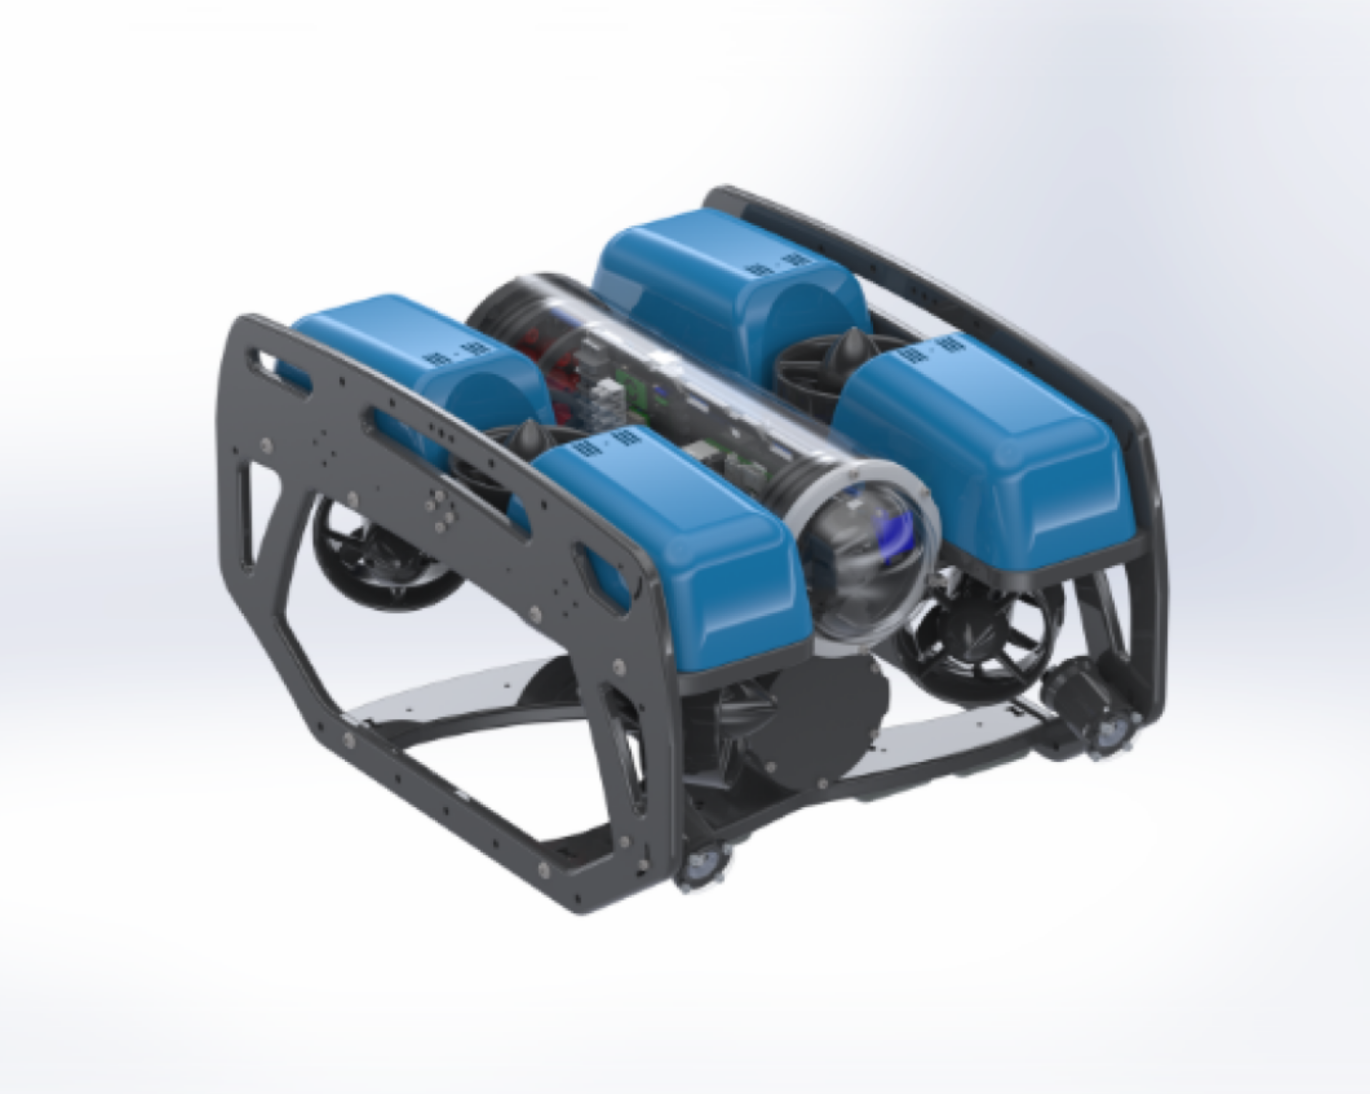
\includegraphics[width=0.6\linewidth]{images/chapter2/bluerov.png}
    \caption{BlueROV2 三维结构}
    \label{f.BlueROV2}
\end{figure}

BlueROV2搭载的传感器可以用于测量系统的状态向量,各传感器技术的测量物理量,采样率和方差如表\ref{t.sensors}所示。
\begin{table}[htb]
  \centering
  \caption{BlueROV2机载传感器参数表}
  \zihao{5}
  
  \label{t.sensors}
  \begin{tabular}{cccc}
  \hline
传感器技术 & 测量状态  & 采样率 & 方差 \\
\hline
压力计 & $z_b$ & 20Hz & $1.5\times 10^{-5}\text{m}$ \\
惯性测量单元 & $\phi, \theta$ & 1000Hz & $1\times 10^{-5}\text{ rad to } 2.5\times 10^{-5}\text{rad}$ \\
磁力计 & $\psi$ & 1000Hz & \multirow{2}{*}{$2\times 10^{-6}\text{m}$} \\
激光照相机 & $x, y$ & 20Hz & \\
短基线技术 & $x_b, y_b$ & 4Hz & $1\times 10^{-3}\text{m}$\\
\hline
\end{tabular}
\end{table}

\section{BlueROV2 运动学建模}
\subsection{坐标系建立与运动参数的定义}

描述 ROV 位置、姿态、速度、加速度之间关系的运动学方程,必须在特定的坐标系下才有意义,用于水下运输的遥控运载机器人的运动可以视为六自由度的运动,一般而言需要建立世界惯性坐标系与运动的载体坐标系用于描述 ROV 的运动参数,两者均满足笛卡尔右手坐标系原则。惯性坐标系的原点取在大地上的一点,Z 轴指向地心,X,Y 轴在水平面内互相垂直,ROV 载体坐标系的原点与 ROV 的重心重合,即:设置 ROV 重心坐标为$r_g=[x_g,y_g,z_g]^T=[0,0,0]^T$,Z 轴指向 ROV 竖直下沉方向,X 轴与 ROV 进退方向平行,指前进方向为正向,Y 轴与 ROV 横移方向平行。根据 BlueROV2 结构,建立惯性坐标系与载体坐标系如图\ref{f.frame_identification}所示。

\begin{figure}[hbt]
    \centering
    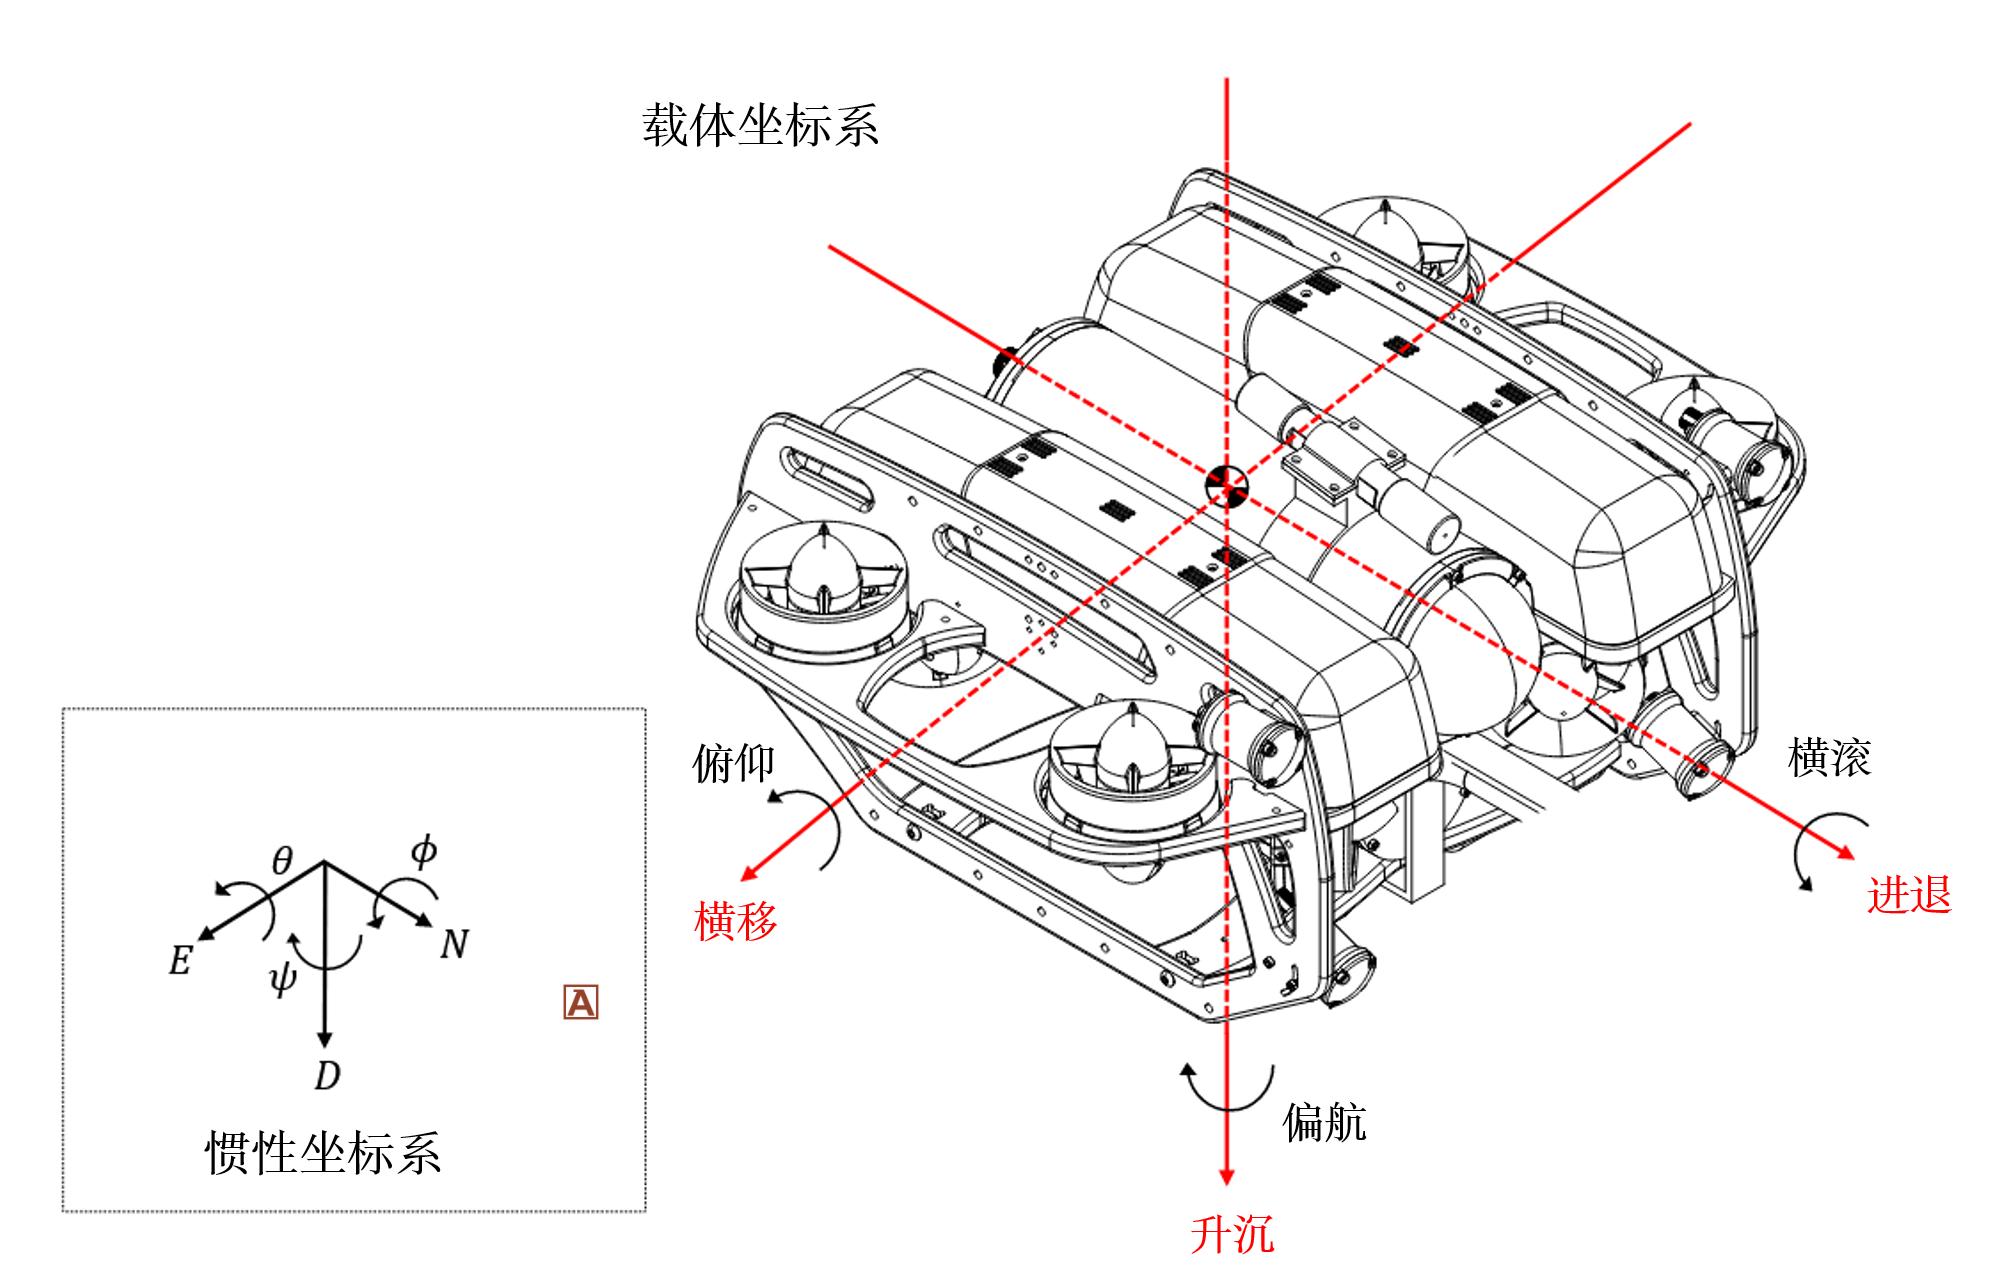
\includegraphics[width=0.8\linewidth]{images/chapter2/frame-identification.png}
    \caption{惯性坐标系与载体坐标系示意图}
    \label{f.frame_identification}
\end{figure}

ROV 的运动位置与姿态一般分别在惯性坐标系和载体坐标系下分别表示。在惯性坐标系下,定义 ROV 的位置向量为$\symbf{\eta}_1 = [x,y,z]^T$,姿态向量为$\symbf{\eta}_2 = [\phi, \theta, \psi]^T$,统称为欧拉角,以$\symbf{\eta} = [\symbf{\eta}_1, \symbf{\eta}_2]=[x,y,z,\phi,\theta,\psi]^T$为惯性坐标系下的广义位姿向量。在载体坐标系下,定义 ROV 沿坐标轴的线速度向量为$\symbf{v}_1 = [u,v,w]^T$,绕坐标轴的角速度向量为$\symbf{v}_2=[p,q,r]^T$,以$\symbf{v} = [\symbf{v}_1,\symbf{v}_2] = [u,v,w,p,q,r]^T$为广义的速度向量。定义 ROV 各方向所受的力沿坐标轴方向的分量组成外力向量$\symbf{\tau}_1=[X, Y, Z]^T$,定义各方向所受力在各坐标轴上产生的力矩为外力矩向量$\symbf{\tau}_2 = [K, M, N]^T$,以$\symbf{\tau}=[\symbf{\tau}_1,\symbf{\tau}_2]=[X, Y, Z ,K, M ,N]^T$为广义受力向量。上述参数的具体定义见表\ref{t.kinetics_params}。

\begin{table}[htb]
  \centering
  \caption{ROV 各坐标系下运动参数定义}
  \zihao{5}
  
  \label{t.kinetics_params}
  \begin{tabular}{cccc}
  \hline
向量 & 惯性坐标系下位姿  & 载体坐标系下速度 & 载体坐标系下受力 \\
\hline
沿$x$轴方向 & $x$  & $u$ & $X$ \\
沿$y$轴方向 & $y$  & $v$ & $Y$ \\
沿$z$轴方向 & $z$  & $w$ & $Z$ \\
绕$x$轴方向 & $\phi$  & $p$ & $K$ \\
绕$y$轴方向 & $\theta$  & $q$ & $M$ \\
绕$z$轴方向 & $\psi$  & $r$ & $N$ \\
\hline
\end{tabular}
\end{table}

\subsection{载体坐标系与惯性坐标系的转换}

在 ROV 的运动控制中,需要对载体坐标系和惯性坐标系下的运动参数进行转换。如 IMU 测得的速度信息往往是在载体坐标系下得到的,而运动控制器所计算的速度信息往往是在惯性坐标系下的速度,因此需要计算两个坐标系之间的转换矩阵,以构建 ROV 的运动学方程。

对于惯性坐标系下的线速度向量$\dot{\symbf{\eta}_1}=[\dot{x},\dot{y},\dot{z}]^T$,角速度向量$\dot{\symbf{\eta}_2} = [\dot{\phi},\dot{\theta},\dot{\psi}]^T$,与惯性坐标系下的线速度向量$\symbf{v}_1=[u,v,w]^T$,角速度向量$\symbf{v}_2=[p,q,r]^T$,他们之间有下列关系:
\begin{equation}
\dot{\symbf{\eta}_1}=\symbf{R}\symbf{v}_1
\label{eq.linear_velocity_trans}
\end{equation}
\begin{equation}
\dot{\symbf{\eta}_2}=\symbf{T}\symbf{v}_2
\label{eq.angular_velocity_trans}
\end{equation}
其中,线速度变换矩阵为:
\begin{equation}
    \symbf{R} = \begin{bmatrix}
        \cos \psi \cos \theta & \sin\psi\sin\theta\sin\phi-\sin\psi\cos\phi & \cos\psi\sin\theta\cos\phi+\sin\psi\sin\phi \\
        \sin\psi\cos\theta & \sin\psi\sin\theta\sin\phi+\cos\psi\cos\phi & \sin\psi\sin\theta\cos\phi-\cos\psi\cos\phi \\
        -\sin\theta & \cos\theta\sin\phi & \cos\theta\cos\phi \\
    \end{bmatrix}
    \label{eq.R_trans}
\end{equation}
对该矩阵求逆,得到:
\begin{equation}
    \symbf{R}^{-1} = \begin{bmatrix}
        \cos\psi\cos\theta & \sin\psi\cos\theta & -\sin\theta \\
        -\sin\psi\cos\theta+\cos\psi\sin\phi\sin\theta & \cos\psi\cos\phi\sin\theta & \cos\theta\sin\phi \\
        -\sin\theta & \cos\theta\sin\phi & \cos\theta\cos\phi \\
    \end{bmatrix}
    \label{eq.R_trans_inv}
\end{equation}
角速度变换矩阵为:
\begin{equation}
    \symbf{T} = \begin{bmatrix}
        1 & \sin\phi\tan\theta & \cos\phi\tan\theta \\
        0 & \cos\phi & -\sin\phi \\
        0 & \sin\phi / \cos\theta & \cos\phi / \cos\theta \\
    \end{bmatrix}
    \label{eq.T_trans}
\end{equation}
对该矩阵求逆,得到:
\begin{equation}
    \symbf{T}^{-1} = \begin{bmatrix}
        1 & 0 & -\sin\theta \\
        0 & \cos\phi & \cos\theta\sin\phi \\
        0 & -\sin\phi & \cos\phi\cos\theta \\
    \end{bmatrix}
    \label{eq.T_trans_inv}
\end{equation}
通过(\ref{eq.linear_velocity_trans}),(\ref{eq.angular_velocity_trans}),(\ref{eq.R_trans}),(\ref{eq.T_trans})联立,可以得到 ROV 运动学方程:
\begin{equation}
    \dot{\symbf{\eta}} = \symbf{J}(\symbf{\eta})\symbf{v}
    \label{eq.kinetics_equation}
\end{equation}
\begin{equation}
    \symbf{J}(\symbf{\eta}) = \begin{bmatrix}
        \symbf{R} & \symbf{0}_{3\times 3} \\
        \symbf{0}_{3\times 3} & \symbf{T} \\
    \end{bmatrix}
    \label{eq.T_trans_inv}
\end{equation}

\section{BlueROV2 动力学模型}

\subsection{电机分布介绍}

BlueROV2 共搭载 6 个 T200 电机,电机分布如图\ref{f.motor_distribution}所示。其中,蓝色推进器为顺时针推进器,绿色推进器为逆时针推进器,红色箭头表示正向前进方向。

\begin{figure}[hbt]
    \centering
    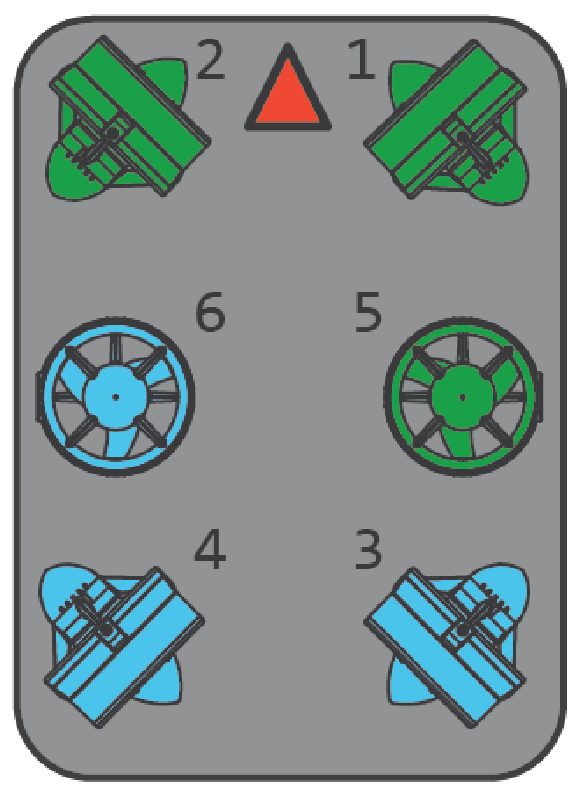
\includegraphics[width=0.2\linewidth]{images/chapter2/motor_distribution.png}
    \caption{BlueROV2 电机分布图}
    \label{f.motor_distribution}
\end{figure}

各电机在载体坐标系下的位置坐标,与电机朝向角度在 BlueROV2 上的设置如表\ref{t.motor_position_rpy}所示。
\begin{table}[htb]
  \centering
  \caption{载体坐标系下的 BlueROV2 电机位置坐标}
  \zihao{5}
  
  \label{t.motor_position_rpy}
  \begin{tabular}{c c c c c c c}
  \hline
电机编号 & X 轴坐标/m  & Y 轴坐标/m & Z 轴坐标/m & 绕 X 旋转/rad & 绕 Y 旋转/rad & 绕 Z 旋转/rad\\
\hline
T1 & 0.1355 & -0.1 & -0.0725 & 0 & 0 & 0.7853 \\
T2 & 0.1355 & 0.1 & -0.0725 & 0 & 0 & -0.7853 \\
T3 & -0.1475 & -0.1 & -0.0725 & 0 & 0 & 2.356\\
T4 & -0.1475 & 0.1 & -0.0725 & 0 & 0 -2.356 & 0\\
T5 & 0.0025 & -0.1105 & -0.005 & 0 & -1.570 & 0\\
T6 & 0.0025 & 0.1105 & -0.005 & 0 & -1.570 & 0\\
\hline
\end{tabular}
\end{table}
BlueROV2 通过 PWM 值控制六个推进器旋转以提供驱动力,通过查询可以得到六个推进器提供推力与 PWM 值呈二次关系,满足:
\begin{equation}
    F = k_1(\text{PWM}-1500)^2 + k_2(\text{PWM}-1500) + k_3
\end{equation}
其中,$F$表示 T200 电机提供推力,$\text{PWM}$表示推进器接收 PWM 值,$k_1,k_2,k_3$表示推力系数。逆时针推进器(正桨)的推力系数满足:
\begin{equation}
    \symbf{k}_\text{正} = [k_1,k_2,k_3]^T = \begin{cases}
  [1.5\times 10^{-6}, 6.0\times 10^{-3} ,7.1\times 10^{-2}], & \text{PWM}>1500 \\
  [0,0,0], & 1460<\text{PWM}<1500, \text{死区} \\
  [-3.3\times 10^{-6}, 6.9\times 10^{-3}, 0.34], & \text{PWM} > 1500 \\
\end{cases}
\end{equation}
顺时针推进器(反桨)的推力系数满足:
\begin{equation}
   \symbf{k}_\text{反} = [k_1,k_2,k_3]^T = \begin{cases}
  [2.5\times 10^{-6}, -5.5\times 10^{-3} ,-0.171], & \text{PWM}>1500 \\
  [0,0,0], & 1470<\text{PWM}<1500, \text{死区} \\
  [-7.9\times 10^{-7}, -7.8\times 10^{-3}, 0.019], & \text{PWM} > 1500 \\
\end{cases}
\end{equation}

\subsection{BlueROV2 受力分析}

在 ROV 的研究与应用中,构建精确的动力学模型是一项具有根本性意义的工作,动力学模型用于描述作用在机器人上的力和力矩与其加速度之间的关系。将 ROV 所受外力进行数学表达是 ROV 动力学建模准确的基础,也是 ROV 运动控制与仿真的前提。

\subsubsection{静力(力矩)}

静力(力矩)是指由于水下航行器自身的重力与所受的浮力共同作用产生的力或力矩。对于 ROV 的重力,一般是将 ROV 的各个部件所受的合力简化到 ROV 主体重心处所受的重力,即重力 $G$ 作用点为重心,类似于重力,ROV 所受的浮力 $B$ 的作用点为浮心。可以得到载体坐标系下的静力方程:
\begin{equation}
    \symbf{g}(\symbf{\eta}) = \begin{bmatrix}
        -(G-B)\sin\theta \\
        (G-B)\cos\theta\sin\phi \\
        (G-B)\cos\theta\cos\phi \\
        -(y_GG-y_BB)\cos\theta\cos\phi + (z_GG-Z_BB)\cos\theta\sin\phi \\
        (z_GG-z_BB)\sin\theta + (x_GG-x_BB)\cos\theta\cos\phi \\
        (x_GG-x_BB)\cos\theta\sin\phi - (y_GG-y_BB)\sin\theta \\
    \end{bmatrix}
    \label{eq.restore_force}
\end{equation}
其中,$x_G,y_G,z_G;x_B,y_B,z_B$分别为 ROV 重心与浮心在载体坐标系下的位置坐标。因为 ROV 载体坐标系原点与重心重合,且 ROV 在浮力配平后,浮心在重心的正上方,所以式(\ref{eq.restore_force})可以简化为
\begin{equation}
    \symbf{g}(\symbf{\eta}) = \begin{bmatrix}
        -(G-B)\sin\theta \\
        (G-B)\cos\theta\sin\phi \\
        (G-B)\cos\theta\cos\phi \\
        -z_BB\cos\theta\sin\phi \\
        -z_BB\sin\theta \\
        0 
    \end{bmatrix}
\end{equation}

\subsubsection{推力器力矩}

图\ref{f.motor_distribution}呈现了 BlueROV2 的推力器分布情况,推进器推力 (力矩) 是指水下机器人安装的螺旋桨或十字舵等推进器提供的驱动力,是 ROV 运动控制策略的执行机构。ROV 的受力向量和推进器提供的推力向量,满足关系
\begin{equation}
     \symbf{\tau} = \symbf{T}\symbf{F}
\end{equation}
其中$\symbf{T}$为推力配置矩阵,满足
\begin{equation}
    \symbf{T} = [\symbf{t}_1, \cdots, \symbf{t}_6]^T
\end{equation}
其中的每个列向量$\symbf{t}_i$将每个推力器产生的力$F_i$与向量$\symbf{\tau}$联系起来:
\begin{equation}
\symbf{t}_i = \begin{bmatrix}
    \symbf{\varepsilon}_i \\
    \symbf{r}_i \times \symbf{\varepsilon}_i
\end{bmatrix}
\end{equation}
其中$\symbf{r}_i$是第$i$个推进器的位置向量,$\symbf{\varepsilon}_i$表示第$i$个推进器的单位推力在三个轴上的分量,定义第$i$个推进器姿态向量为$\symbf{\eta}_{mi}=[\phi_i, \theta_i, \psi_i]^T$,则
\begin{equation}
    \symbf{\varepsilon}_i=[\cos\psi_i\cos\theta_i,\sin\psi_i\cos\theta_i,-\sin\theta_i]
\end{equation}
通过代入各个推进器的姿态向量,可以计算出BlueROV2的推力配置矩阵$\symbf{T}$。
\begin{equation}
    \symbf{T} = \begin{bmatrix}
        0.707 & 0.707 & -0.707 & -0.707 & 0 & 0\\
        -0.707 & 0.707 & -0.707 & 0.707 & 0 & 0 \\
         0 & 0 & 0 & 0 & 1 & 1 \\
         0.051 & -0.051 & 0.051 & -0.051 & 0.111 & -0.111 \\
         0.051 & 0.051 & -0.051 & -0.051 & 0.002 & -0.002 \\
         -0.167 & 0.167 & 0.175 & -0.175 & 0 & 0 \\
    \end{bmatrix}
\end{equation}

\subsubsection{水动力建模}

水动力是指ROV在水下航行过程中周围流体的反作用力,主要包括惯性水动力与粘性水动力。水动力的产生根源在于ROV与周围水体之间的相互作用,影响ROV所受水动力的因素有很多,主要包括ROV的几何外形,航行速度、加速度与流体物理属性的影响。在一般水下作业下,本文假设ROV几何外形基本不变,流体物理属性基本保持一致,以此将ROV的水动力方程简化为ROV速度、加速度的函数。

惯性水动力$F_I(\dot{V})$满足
\begin{equation}
    F_I(\dot{V})=\lambda_{ij}\dot{V}
\end{equation}
其中,$\dot{V}$表示ROV在载体坐标系下的加速度,比例系数$\lambda_{ij}$为附加质量系数。

粘性水动力$F_D(V)$满足
\begin{equation}
    F_D(V) = q_{ij}V
\end{equation}
其中,$V$表示ROV在载体坐标系下的速度,比例系数$q$为一阶阻尼系数。

\subsubsection{其他受力}

ROV在水下航行作业时,其运动状态和控制精度会受到复杂且动态变化的水下环境带来的各种干扰力的影响。这些力来源广泛,既有外部环境因素,也有ROV本体自身特性与环境交互产生的因素。水体环境的复杂多变,会导致动力学模型存在噪音,设由环境产生的非结构性受力为$\symbf{\tau}_e$。

\section{BlueROV2 动力学建模}

鉴于ROV的水下航行可以视为刚体六自由度运动,使用刚体牛顿-欧拉运动方程对ROV进行运动学建模,动力学方程如下:
\begin{equation}
    \symbf{M}\dot{\symbf{V}}+\symbf{C}(\symbf{v})+\symbf{D}(\symbf{v})+\symbf{g}(\symbf{\eta}) = \symbf{\tau} + \symbf{\tau}_e
\end{equation}
其中,$\symbf{M} = \symbf{M}_{RB}+\symbf{M}_a$,分别为ROV的刚体质量矩阵和附加质量矩阵;$\symbf{C}(\symbf{v})=\symbf{C}_{RB}(\symbf{v})+\symbf{C}_a(\symbf{v})$,分别为ROV的刚体科里奥利力矩阵和附加科里奥利力矩阵;$\symbf{D}(\symbf{v})=\symbf{D}_l(\symbf{v})+\symbf{D}_q(\symbf{v})$,分别为ROV所受的一阶流体阻力和二阶流体阻力;$\symbf{g}(\symbf{\eta})$为ROV所受重力与浮力共同组成的恢复力,即上文所提到的静力(力矩);$\symbf{\tau}$为6个电机提供的驱动力与驱动力矩;$\symbf{\tau}_e$为ROV在水下航行过程中由于环境等不可控因素导致的受力。

上述动力学方程中,ROV的质量矩阵满足$\symbf{M}_{RB}=\symbf{M}_{RB}^T>0$,满足
\begin{equation}
    \symbf{M}_{RB}=\begin{bmatrix}
        m\symbf{I}_{3\times 3} & -mS(r_g^b) \\
        mS(r_g^b) & \symbf{I}_b \\
    \end{bmatrix} = \begin{bmatrix}
        m & 0 & 0 & 0 & mz_g & -my_g \\
        0 & m & 0 & -mz_g & 0 & mx_g \\
        0 & 0 & m & my_g & -mx_g & 0 \\
        0 & -mz_g & my_g & I_x & -I_{xy} & -I_{xz} \\
        mz_g & 0 & -mx_g & -I_{yx} & I_y & -I_{yz} \\
        -my_g & mx_g & 0 & -I_{zx} & -I_{zy} & I_z \\
    \end{bmatrix}
\end{equation}
其中,$m$为ROV质量,$r_g^b = [x_g,y_g,z_g]^T$为载体坐标系下的质心的位置坐标,由于载体坐标系下原点与ROV的质心重合,故$r_g^b=[0,0,0]^T$;上式中
 $$I_x = \int_V(y^2+z^2)\rho_mdV$$
 $$I_y = \int_V(x^2+z^2)\rho_mdV$$
 $$I_z = \int_V(x^2+y^2)\rho_mdV$$
 $$I_xy = \int_Vxy\rho_mdV=I_{yx}$$
 $$I_xz = \int_Vxz\rho_mdV=I_{zx}$$
\begin{equation}
 I_yz = \int_Vyz\rho_mdV=I_{zy}
\end{equation}
设三条坐标轴为中心惯性主轴,则$I_{xy} = I_{yz} = I_{xz} = 0$,$\symbf{I_b} = diag([I_x, I_y, I_z])$;$S(\cdot)$为矢量相乘算子,满足:
$$\symbf{\lambda}\times \symbf{a}:=\symbf{S}(\symbf{\lambda})\symbf{a}$$
\begin{equation}
    \symbf{S}(\symbf{\lambda})=-\symbf{S}^T(\symbf{\lambda})=\left[
    \begin{matrix}
    0 & -\lambda_3 & \lambda_2 \\
    \lambda_3 & 0 & -\lambda_1 \\
    -\lambda_2 & \lambda_1 & 0 \\
    \end{matrix}
    \right], \symbf{\lambda}=\left[
    \begin{matrix}
    \lambda_1 \\
    \lambda_2 \\
    \lambda_3 \\
    \end{matrix}
    \right]
\end{equation}
由此可以得到刚体质量矩阵的表达式
\begin{equation}
    \symbf{M}_{RB} = \begin{bmatrix}
        m\symbf{I}_{3\times 3} & -mS(r_g^b) \\
        mS(r_g^b) & \symbf{I}_b \\
    \end{bmatrix} = \begin{bmatrix}
    m & 0 & 0 & 0 & 0 & 0 \\
    0 & m & 0 & 0 & 0 & 0 \\
    0 & 0 & m & 0 & 0 & 0 \\
    0 & 0 & 0 & I_x & 0 & 0 \\
    0 & 0 & 0 & 0 & I_y & 0 \\
    0 & 0 & 0 & 0 & 0 & I_z \\
\end{bmatrix}
\end{equation}
附加质量矩阵满足
\begin{equation}
    \symbf{M}_a = diag([X_{\dot{u}},Y_{\dot{v}},Z_{\dot{w}},K_{\dot{p}},M_{\dot{q}},N_{\dot{r}}])
\end{equation}
其中,$X_{\dot{u}},Y_{\dot{v}},Z_{\dot{w}},K_{\dot{p}},M_{\dot{q}},N_{\dot{r}}$为ROV附加质量系数。

对质量矩阵进行处理
\begin{equation}
\symbf{M} = \begin{bmatrix}
    \symbf{M}_{11} & \symbf{M}_{12} \\
    \symbf{M}_{21} & \symbf{M}_{22} \\
\end{bmatrix}    
\end{equation}
可以得到科里奥利力矩阵$\symbf{C}(\symbf{v})$为:
\begin{equation}
    \symbf{C}(\symbf{v}) = \begin{bmatrix}
        \symbf{0}_{3\times 3} & -S(\symbf{M}_{11}\symbf{v}_1+\symbf{M}_{12}\symbf{v}_2) \\ 
        -S(\symbf{M}_{11}\symbf{v}_1+\symbf{M}_{12}\symbf{v}_2) & -S(\symbf{M}_{21}\symbf{v}_1+\symbf{M}_{22}\symbf{v}_2)
    \end{bmatrix}
\end{equation}
其中,$\symbf{v}_1 = [u,v,w]^T,\symbf{v}_2=[p,q,r]^T$,由此可以得到科里奥利力矩阵的表达式
\begin{equation}
    \symbf{C}_{RB}(\symbf{v})=
\begin{bmatrix}
    0 & 0 & 0 & 0 & mw & -mv \\
    0 & 0 & 0 & -mw & 0 & mu \\
    0 & 0 & 0 & mv & -mu & 0 \\
    0 & mw & -mv & 0 & I_zr & -I_yq \\
    -mw & 0 & mu & -I_zr & 0 & I_xp \\
    mv & -mu & 0 & I_yq & -I_xp & 0 \\
\end{bmatrix}
\end{equation}

\begin{equation}
    \symbf{C}_a(\symbf{v})=
\begin{bmatrix}
    0 & 0 & 0 & 0 & -Z_{\dot{w}}w & Y_{\dot{v}}v \\
    0 & 0 & 0 & Z_{\dot{w}}w & 0 & -X_{\dot{u}}u \\
    0 & 0 & 0 & -Y_{\dot{v}}v & X_{\dot{u}}u & 0 \\
    0 & -Z_{\dot{w}}w & Y_{\dot{v}}v & 0 & -N_{\dot{r}}r & M_{\dot{q}}q \\
    Z_{\dot{w}}w & 0 & -X_{\dot{u}}u & N_{\dot{r}}r & 0 & -K_{\dot{p}}p \\
    -Y_{\dot{v}}v & X_{\dot{u}}u & 0 & -M_{\dot{q}}q & K_{\dot{p}}p & 0 \\
\end{bmatrix}
\end{equation}
ROV所受的一阶水动力阻尼和二阶水动力阻尼可分别用(\ref{eq.linear_damping}),(\ref{eq.square_damping})表示
\begin{equation}
    \symbf{D}_l=-diag([X_u,Y_v,Z_w,K_p,M_q,N_r])
    \label{eq.linear_damping}
\end{equation}
\begin{equation}
    \symbf{D}_{q}(\symbf{v}) = -diag([X_{u|u|}|u|,Y_{v|v|}|v|,Z_{w|w|}|w|,K_{p|p|}|p|,M_{q|q|}|q|,N_{r|r|}|r|])
    \label{eq.square_damping}
\end{equation}
其中,$X_u,Y_v,Z_w,K_p,M_q,N_r$为一阶水阻尼系数,$X_{u|u|},Y_{v|v|},Z_{w|w|},K_{p|p|},M_{q|q|},N_{r|r|}$为二阶水阻尼系数。

至此,本文获得简化后的BlueROV2动力学方程,方程中相关物理信息可以通过实际测量得到,见表\ref{t.physical_params}所示。

\begin{table}[htb]
  \centering
  \caption{BlueROV2物理参数表}
  \zihao{-5}
  \label{t.physical_params}
  \begin{tabular}{c c c c c c c c}
  \hline
参数名 & 质量($m$) & 惯性矩($I_x$)& 惯性矩($I_y$) & 惯性矩($I_z$) & 重力($G$) & 浮力($B$) & 浮心$z$轴坐标  \\
\hline
参数值 & 11.2 & 0.303 & 0.626 & 0.576 & 112.80 & 111.47 & 0.02 \\
单位 & $kg$ & $kg\cdot m^2$ & $kg\cdot m^2$ & $kg\cdot m^2$ &  N & N & m \\
\hline
\end{tabular}
\end{table}

\subsection{本章小结}

本章围绕BlueROV2的运动学与动力学建模展开了详细的论述。首先介绍了ROV的结构设计特点,为后续的建模分析奠定了基础。在运动学建模部分,重点明确了坐标系的建立规则和运动参数的定义,并详细推导了载体坐标系与惯性坐标系之间的转换关系,用于描述ROV空间位姿与运动参数的关系。随后,章节深入到BlueROV2的动力学模型构建,首先概述了其电机的分布情况,接着对BlueROV2进行了全面的受力分析,具体探讨了作用在ROV上的静力、推进器产生的推力与力矩、复杂的水动力以及其他可能的环境扰动力。在分别对各项力进行建模和分析的基础上,最终整合形成了BlueROV2的完整动力学方程,为后续的仿真分析、控制器设计以及运动特性研究提供了数学依据和理论支持。

\newpage
